\section{Zielsetzung}
Mit der Hilfe von Brückenschaltungen lässt sich jede physikalische Größe, die sich
eindeutig als Widerstand darstellen lässt messen.
Dies wird mit verschiedenen Arten von Brückenschaltungen durchgeführt.

\section{Theorie}
Allgemein wird bei Brückenschaltungen die Potentialdifferenz zwischen zwei
Punkten zweier getrennter stromduchflossener Leiter in Abhängigkeit des
Widerstandsverhältnisses gemessen. Daher hat sie im allgemeinen eine Schaltung wie in
Abbildung \ref{fig:allg} dargestellt.
\begin{figure}[H]
  \centering
  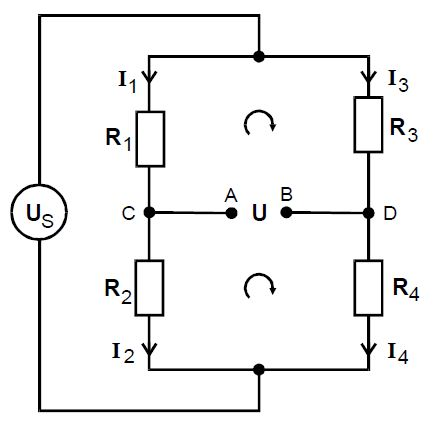
\includegraphics[height=5cm]{allg.JPG}
  \caption{Allgemeine Schaltung einer Brückenschaltung}
  \label{fig:allg}
  \cite{skript}.
\end{figure}
\noindent Als Brückenspannung wird die zwischen den Punkten A und B auftretende Spannung
bezeichnet. Sie lässt sich mit Hilfe der Kirchhoffschen Gestze berechnen.
Dabei lautet das 1. Kirchhoffsche Gesetz: In einem Knotenpunkt muss die
Summe aus allen Strömen (zufließend und abfließend) Null ergeben.
\begin{equation}
  \sum_{i} I_{i} = 0
  \label{eqn:kirch1}
\end{equation}
Das zweite Kirchhoffsche Gesetz lautet: In jeder Masche eines Stromkreises
ist die Summe über die Spannungen gleich Null.
\begin{equation}
  \sum_{i} U_{i} =0
  \label{eqn:kirch2}
\end{equation}

\noindent Aus diesen Gesetzen lässt sich folgender Zusammenhang für die Brückenspannung
herleiten:
\begin{equation}
  U=\frac{R_{2}R_{3}-R_{1}R_{4}}{(R_{3}+R_{4})(R_{1}+R_{2})}U_{S}.
  \label{eqn:ubrücke}
\end{equation}
\noindent Hieran lässt sich erkennen, dass die Brückenspannung für die Bedingung
\begin{equation}
  R_{2}R_{3}=R_{1}R_{4}
  \label{eqn:rbrücke}
\end{equation}
verschwindet. Ist das der Fall, wird die Brücke als abgeglichene Brücke bezeichnet.
Da die Abgleichbedingung nur von den Widerständen abhängig ist, kann durch
variieren dreier bekannter Widerstände (z.B. $R_{2}$,$R_{3}$,$R_{4}$) ein unbekannter
Widerstand (z.B. $R_{1}$) ausgemessen werden. Die Genauigkeit der Messung ist davon
abhängig, wie genau die Widerstände (z.B. $R_{2}$,$R_{3}$,$R_{4}$) bekannt sind und wie
ganau der Wert "Null" als Brückenspannung eingestellt werden kann.
Die Abgleichbedingung ist unabhängig von der Speisespannung $U_{S}$, da
die Brückenspannung aber proportional zu dieser ist, sollte sie
dennnoch hoch gewählt werden, um eine hohe Abgleichempfindlichkeit zu erhalten.

\noindent Enthält die Brückenschaltung auch Kapazitäten und
Induktivitäten, dann werden für die Berechnung komplexe
Widerstände, auch Impedanzen genannt verwendet. Diese haben die allgemeine Form
\begin{equation}
  Z = X + iY,
\end{equation}
wobei $X$ der Wirkwiderstand und $Y$ der Blindwiderstand ist. Für einen
Kondensator $C$, eine Induktivität $L$, und eine ohmschen Widerstand $R$
ergeben sich folgende Impedanzen.
\begin{align*}
  Z_{C} &= \frac{-i}{\omega C} \\
  Z_{L} &= i \omega L\\
  Z_{R} &= R\\
\end{align*}

\noindent Für eine Brückenschaltung mit Impedanzen lautet die Abgleichbedingung äquivalent zu
Gleichung \ref{eqn:rbrücke}:
\begin{equation}
  Z_{2}Z_{3}=Z_{1}Z_{4}.
  \label{eqn:zbrücke}
\end{equation}
\noindent Imaginäre Zahlen sind im Allgemeinen genau dann gleich, wenn der Real- und
Imaginärteil gleich sind. Daher muss für eine abgeglichene Wechselspannungsbrücke
die Brückenspannung nach Betrag und Phase verschwinden.
Deshalb besitzt jede Wechselstrombrücke zwei voneinander unabhängige Stellglieder.

\subsection{Wheatstonsche Brücke/Widerstandsmessbrücke}
\noindent Diese Brückenschaltung kann mit Gleich- und Wechselstrom betrieben werden,
da sie nur ohmsche Widerstände enthält.
\begin{figure}[H]
  \centering
  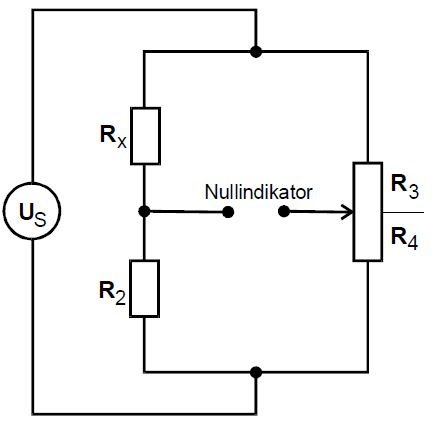
\includegraphics[height=5cm]{widerstand.JPG}
  \caption{Wheatstonsche Brückenschaltung}
  \label{fig:widerstand}
  \cite{skript}.
\end{figure}

\noindent Mit dieser Schaltung kann der unbekannte Widerstand $R_{x}$ gemessen werden.
Nach Gleichung \ref{eqn:rbrücke} gilt die Bedingung
\begin{equation}
  R_{x}= R_{2}\frac{R_{3}}{R_{4}}.
  \label{eqn:rx}
\end{equation}
$R_{x}$ ist von dem Verhältnis von $R_{3}$ zu $R_{4}$ abhängig. Dieses Bauteil, dessen
Widerstand stufenlos verstellbar ist, wird auch als Potentiometer bezeichnet.
\subsection{Kapazitätsmessbrücke}
Da es in einem realen Kondensator durch die Umwandlung von elektrischer Energie in
Wärme zu dielektrischen Verlusten kommt, wird ein Ersatzschaltbild eingeführt.
In diesem Ersatzschaltbild wird der Kondensator mit einem (fiktiven) ohmschen Widerstand
in Reihe geschaltet. Somit ergibt sich für einen realen Kondensator:
\begin{equation*}
  Z_{C_{\text{real}}}=R-\frac{i}{\omega C}.
  \label{eqn:zcreal}
\end{equation*}
\begin{figure}[H]
  \centering
  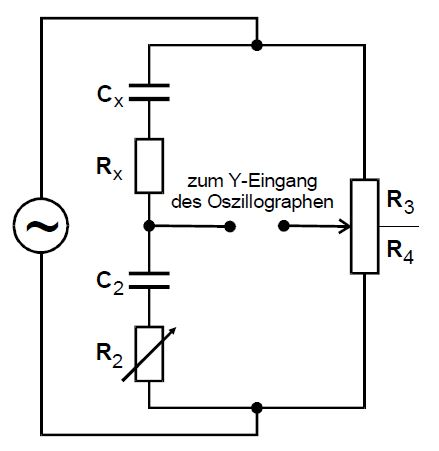
\includegraphics[height=5cm]{kapazitat.JPG}
  \caption{Kapazitätsmessbrücke für Kondensatoren mit dielektrischen Verlusten}
  \label{fig:kapazitat}
  \cite{skript}.
\end{figure}
\noindent Mit dieser Brücke kann eine unbekannte Kapazität $C_{x}$ gemessen werden.
Dabei ist neben dem Potentiometer auch der Widerstand
$R_{2}$ veränderlich.
Aus der Abgleichbedingung \ref{eqn:zbrücke} ergibt sich
\begin{align}
  R_{x} &=R_{2}\frac{R_{3}}{R_{4}} \;\;\;\;\text{und} \\
  C_{x} &=C_{2}\frac{R_{4}}{R_{3}}.
  \label{eqn:cx}
\end{align}

\subsection{Induktivitätsmessbrücke}
 Auch eine reale Induktivität wandelt einen Teil der Enrgie in Wärme um, daher wird äquivalent
 zum Kondensator ein Ersatzschaltbild eingeführt, in dem ein ohmscher Widerstand in Reihe
 zur Induktivität geschaltet wird.
 Daraus ergibt sich für die Impedanz einer realen Spule:
 \begin{equation}
   Z_{L_{\text real}}= R + i\omega L.
   \label{zlreal}
 \end{equation}

\begin{figure}[H]
  \centering
  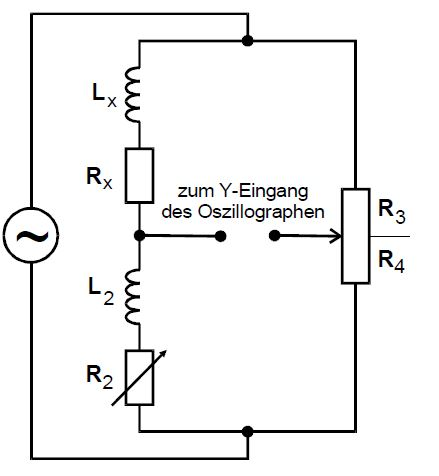
\includegraphics[width=7cm,height=6cm]{induktivitat.JPG}
  \caption{Messbrücke für reale Induktivitäten.}
  \label{fig:induktivitat}
  \cite{skript}
\end{figure}
\noindent Aus der Abgleichbedingung \ref{eqn:zbrücke} ergibt sich
\begin{align}
  R_{x} &=R_{2}\frac{R_{3}}{R_{4}} \;\;\;\; \text{und} \\
  L_{x} &=L_{2}\frac{R_{3}}{R_{4}}.
  \label{eqn:lx}
\end{align}

\noindent In dieser Schaltung sollte die Induktivität $L_{2}$ möglichst geringe
Verluste besitzen und der Wirkanteil sollte nur durch den Widerstand $R_{2}$ erzeugt werden.
Diese Forderungen sind bei niedrigen Frequenzen schwer zu realisieren, weshalb
sattdessen häufig die Maxwell-Brücke verwendet.

\subsection{Maxwell-Brücke}
\noindent In der Maxwellbrücke dienen die Widerstände $R_{3}$ und $R_{4}$ als Abgleichelemente,
$R_{2}$ ist ein bekannter Widerstand.

\begin{figure}[H]
  \centering
  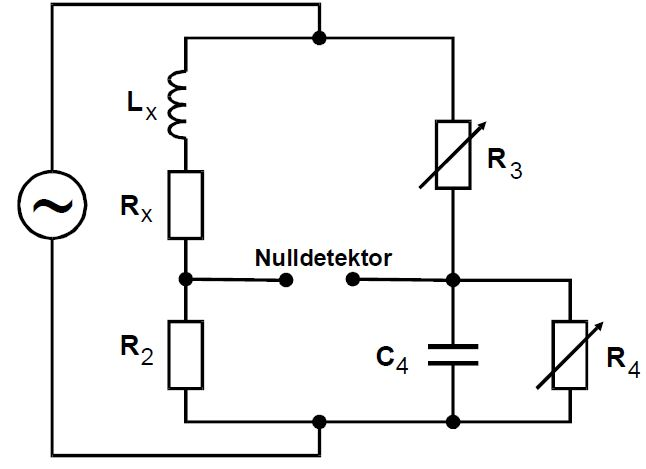
\includegraphics[width=8cm,height=6cm]{maxwell.JPG}
  \caption{Maxwell-Brücke zur untersuchung realer Induktivitäten.}
  \label{fig:maxwell}
  \cite{skript}
\end{figure}

\noindent Aus den Abgleichbedingungen \ref{eqn:zbrücke} folgt:
\begin{align}
  R_{x} &=\frac{R_{2} R_{3}}{R_{4}} \;\;\;\; \text{und} \\
  L_{x} &=R_{2}R_{3}C_{4}.
  \label{eqn:mx}
\end{align}

\noindent In den bisher vorgestellten Brückenschaltugen sind die Abgleichbedingungen
unabhängig von der Frequenz der Speisespannung. Theoretisch sollten sich die Brücken bei jeder
Frequenz abgleichen lassen, in der Praxis gibt es jedoch einen Frequenzbereich in dem
dies besonders gut funktioniert, dieser muss im Experiment ermittelt werden.
Bei zu hohen Frequenzen wird der Einfluss der Streukapazitäten zu hoch, während
bei zu niedrigen Frequenzen aufgrund der Einschwingvorgänge mehrere Periodendauern
gewarten werden muss, bis sich eine stabile Brückenspannung einstellt.
Der optimale Frequenzbereich ist, wenn die Blind- und Wirkwiderstände in der
Schaltung die gleiche Größenordnung besitzen.

\subsection{Frequenzabhängige Brückenschaltung - Wien-Robinson-Brücke}
Diese Brücke ist frequenzabhängig und enthält im Vergleich zu den bisherigen Brücken
keine Abgleichelemente.
\begin{figure}[H]
  \centering
  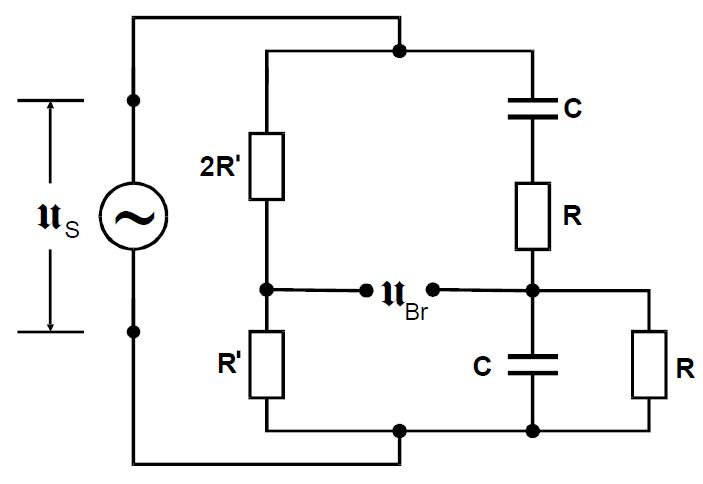
\includegraphics[width=8cm,height=6cm]{wien.JPG}
  \caption{Schaltbild der Wien-Robinson-Brücke}
  \label{fig:wien}
  \cite{skript}.
\end{figure}

\noindent Aus den Gleichungen \ref{eqn:ubrücke} und \ref{eqn:zbrücke} erhält man,
dass die Brückenspannung genau für
\begin{equation*}
  \omega_{0}=\frac{1}{RC}
  \label{eqn:omega}
\end{equation*}
verschwindet.
Zur Vereinfachung wird das Frequenzverhältnis $\Omega=\frac{\omega}{\omega_{0}}$
eingefürhrt. Damit ergibt sich für das Verhältnis von Speise- zu Brückenspannung:
\begin{equation}
  \Bigl|\frac{U_{Br}}{U_{s}}\Bigr|=\frac{((\Omega)^2-1)^2}{9(1-(\Omega)^2)^2+9(\Omega)^2}.
  \label{eqn:betrag}
\end{equation}
An dieser Gleichung \ref{eqn:betrag} wird deutlich, das die Wien-Robinson-Brücke
die Funktion eines elektrischen Filters hat. Sie filtert aus einem kontiniuierlichem
Spektrum alle Wellen der Frequenz $\omega_{0}=\frac{1}{RC}$ heraus.

\noindent Mit dieser Brücke kann eine sogenannte Klirrfaktormessung durchgeführt werden.
Der Kirrfaktor gibt an, in welchem Maß die Grundschwingung von Oberwellen überlagert
wird. Eine Sinusschwingung sollte eigentlich keine Oberwellen besitzen, doch mit realen
Sinusgeneratoren ist dies nur schwer zu realisieren. Der Klirrfaktor dient deshalb
als Maß für die Qualität eines Sinusgenerators.
Um den Klirrfaktor zu messen, wird am Sinusgenerator die Sperrfrequenz $\omega_{0}$
der Wien-Robinson-Brücke eingestellt wird. Somit bleiben nur die von $\omega_{0}$
verschiedenen Frequenzen übrig.

\subsection{Frequenzabhängige Brückenschaltung - TT-Brücke}
Die TT-Brücke ist ebenfalls frequenzabhängig und hat wie die Wien-Robinson-Brücke
die Funktion eines elektrischen Filters.

\begin{figure}[H]
  \centering
  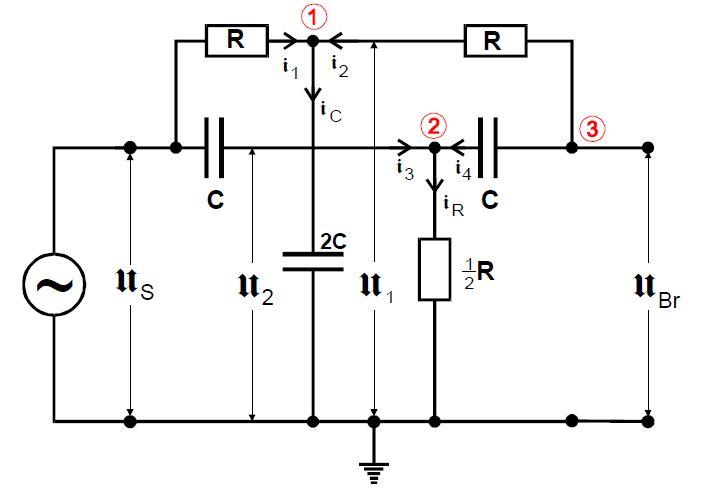
\includegraphics[width=8cm,height=6cm]{tt.JPG}
  \caption{Schaltung einer TT-Brücke}
  \label{fig:tt}
  \cite{skript}.
\end{figure}

\noindent Der Vorteil dieser Schaltung ist, dass die Brückenspannung $U_{Br}$ und auch
die Speisespannung $U_{S}$ gegen Masse angeschlossen werden können.
Mit Hilfe der Kirchhoffschen Gesetze erhält man folgenden Ausdruck für die
Brückenspannung
\begin{equation}
  U_{Br}=U_{S}\frac{1-\omega^2 R^2C^2}{1-\omega^2 R^2C^2-4i\omega RC}.
  \label{eqn:ubr}
\end{equation}
Für die Frequnz $\omega=\frac{1}{RC}$ verschwindet die Brückenspannung. Mit der
Relation $\Omega=\frac{\omega}{\omega_{0}}$ ergibt sich
\begin{equation}
  \Bigl|\frac{U_{Br}}{U_{s}}\Bigr|^2=\frac{(1-\Omega^2)^2}{(1-\Omega^2)^2+16\Omega^2}.
\end{equation}
Es sind viele Ähnlichkeiten zur Wien-Robinson-Brücke erkennen.



\label{sec:Theorie}

%\cite{sample}
